\subsection{Digitale Transformation mit Internet of Things}
Hier könnte man Bezug auf Energiesektor (kurz) nehmen und einführen, mit welchen Anforderungen und technologien generell so ein Wandel/Transformation statfinden kann.
\begin{itemize}
  \item Disruption bestehender Geschäftsmodelle, vom Produzenten zum Dienstleister \citep{Doleski2017}
  \item wichtige Rolle kommunaler Unternehmen als Bereitsteller von Infrastrukturen wie Strom, Gas, Wärme, Wasser, Abwasser, Abfallwirtschaft, Stadtreinigung, Breitband \citep{Doleski2017}
  \item Beitrag zu funktionierendem Gemeinwesen, sozialer Teilhabe und Versorgungssicherheit -> Partner erster Wahl beim Gelingen der digitalen Transformation
  \item Wichtig für Gelingen: Erfahrungsaustausch, Kooperationen, richtige politische Rahmenbedingungen -> Katherine Reiche
  \item auf Unternehmensseite: Aufbau und Umsetzung einer unternehmensspezifischen Digitalisierungsstrategie: RAMI 4.0 als Referenz möglich
  \item Drei Revolutionen in der Energiewirtschaft \citep{Doleski2017}
  \begin{enumerate}
    \item Ab 1998: Liberalisierung und Privatisierung der Strommärkte fördert Wettbewerb, stellt aber eine Herausforderung Digitalisierungsstrategie
    \item Ab 2011: Energiewende und Aussteig aus Kernenergie fördert neue Technologien für erneuerbare Energien, aber die Berechenbarkeit der Kapazitäten verändert sich
    \item Digitalisierung: Potenzial für neue Revolution, Strom kann zwar nicht digitalisiert werden, aber die Vertriebsmodelle
  \end{enumerate}
  \item Datenschutz und Sicherheit gewinnen an Bedeutung
  \item Trend: Energieversorgungsunternehmen wandeln sich Richtung Dienstleitsungsunternehmen
  \item \glqq Mit der Zunahme dezentraler Einspeisungs- und Eigenversorgungsanlagen innerhalb der bestehenden Strom- und Gasnetze steigen synchron auch die Koordinationsanforderungen und die zu beherrschenden Datenmengen \grqq{} \citep[S. 7]{Doleski2016}
  \item \glqq Bedarf einer branchenweiten Veränderung - einer Transformation - in allen Sektoren und Phasen entlang der energiewirtschaftlichen Wertschöpfung\grqq{} \cite[S. 11]{Doleski2016}
  \item Utility 4.0: Digitale Enegergiedienstleistungsunternehmen
  \item Während nach Dampfmaschine, Massenproduktion und Automation nunmehr die Digitalisierung die vierte industrielle Revolution einläutet, unterliegt die Energiewirtschaft ähnlichen Entwicklungsprozessen.
\end{itemize}

\begin{figure}[ht]
  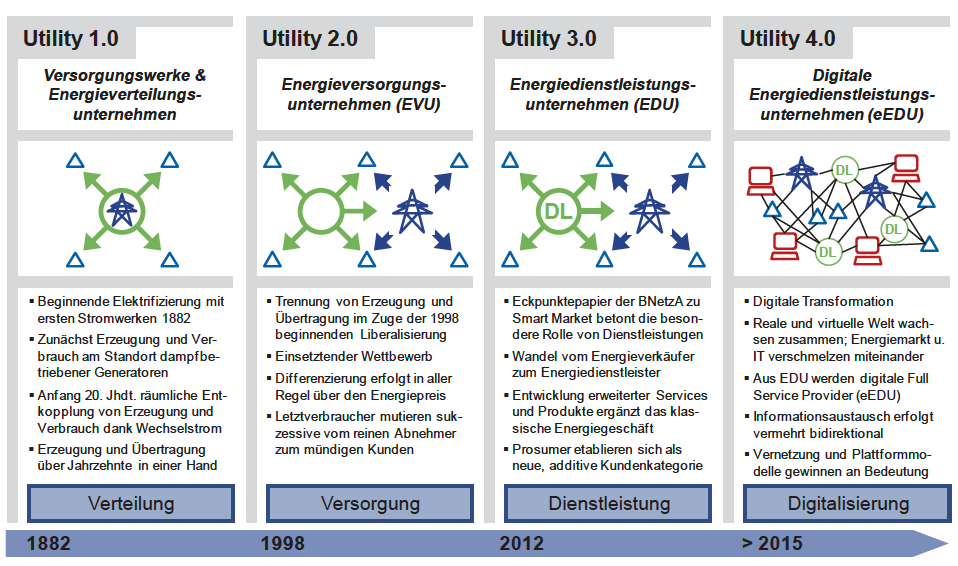
\includegraphics[width=1.0\linewidth]{utility_40.png}
  \caption[Transformation vom Versorgungswerk zum digitalen Energiedienstleister]{Transformation vom Versorgungswerk zum digitalen Energiedienstleister \citep[S. 13]{Doleski2016}}
\end{figure}

\begin{figure}[ht]
  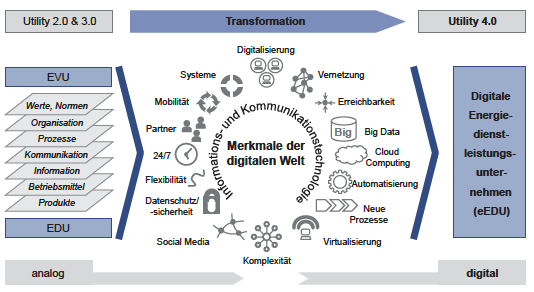
\includegraphics[width=1.0\linewidth]{kalalysator_utility_40.png}
  \caption[Digitale Welt als Katalysator für Utility 4.0 ]{Digitale Welt als Katalysator für Utility 4.0 \citep[S. 17]{Doleski2016}}
\end{figure}

\subsubsection{Anforderungen an ein IoT-System}
nach RAMI 4.0
RAMI (Referenzarchitekturmodell Industrie) 4.0: OPC-UA: Kommunikationsstandards (inkl. Sicherheit)
Sensorik: Bedeutung und sehr oberflächlich Funktionsweisen beschreiben
Gateways: Edge Processing
Device Management
Digital Twins

\subsubsection{Cloud Computing}
Cloud-Native-Development -> neues Paradigma fernab vom 3-Thier Modell
IaaS, PaaS, SaaS, Microservices/SOA: service-oriented architecture
Integration modularer Services!= monolithische Strukur
Integration heterogener Datenquellen
